%%%%%%%%%%%%%%%%%%%%%%%%%%%%%%%%%%%%%%%%%%%%%%%%%%%%%%
% A Beamer template for HKUST (GZ)                   %
% Based on THU beamer theme                          %
% Author: Yuxuan HU                                  %
% Date: Aug 2024                                    %
% LPPL Licensed.                                     %
%%%%%%%%%%%%%%%%%%%%%%%%%%%%%%%%%%%%%%%%%%%%%%%%%%%%%%

\documentclass[serif, aspectratio=169]{beamer}
%\documentclass[serif]{beamer}  % for 4:3 ratio
\usepackage[T1]{fontenc} 
\usepackage{fourier} % see "http://faq.ktug.org/wiki/uploads/MathFonts.pdf" for other options
\usepackage{hyperref}
\usepackage{latexsym,amsmath,xcolor,multicol,booktabs,calligra}
\usepackage{graphicx,pstricks,listings,stackengine}
\usepackage{lipsum}

\author{Azizul Haque Tutul (214052)}
\title{The Impact of AI on Education Today
}
\subtitle{AI in Education}
\institute{
  Email:azizulhaquetutul3695@gmail.com \\
    Department of Computer Science and Engineering \\
    Dhaka University of Engineering \& Technology, Gazipur}\\
\\
}
\date{\small \today}
\usepackage{HKUSTstyle}

% defs
\def\cmd#1{\texttt{\color{red}\footnotesize $\backslash$#1}}
\def\env#1{\texttt{\color{blue}\footnotesize #1}}
% set colors
\definecolor{hkustyellow}{RGB}{167, 131, 55}
\definecolor{hkustblue}{RGB}{0, 56, 116}
\definecolor{hkustred}{RGB}{209, 51, 59}


\lstset{
    basicstyle=\ttfamily\small,
    keywordstyle=\bfseries\color{deepblue},
    emphstyle=\ttfamily\color{deepred},    % Custom highlighting style
    stringstyle=\color{deepgreen},
    numbers=left,
    numberstyle=\small\color{halfgray},
    rulesepcolor=\color{red!20!green!20!blue!20},
    frame=shadowbox,
}

% Footer setting
\setbeamertemplate{footline}{
  \leavevmode%
  \hbox{%
    \begin{beamercolorbox}[wd=.75\paperwidth, ht=2.25ex, dp=1ex, center]{author in head/foot}%
      \usebeamerfont{author in head/foot}Azizul Haque Tutul%
    \end{beamercolorbox}%
    \begin{beamercolorbox}[wd=.25\paperwidth, ht=2.25ex, dp=1ex, center]{title in head/foot}%
      \usebeamerfont{title in head/foot}\insertshorttitle%
    \end{beamercolorbox}%
  }%
  \vskip0pt%
}

%- --- --- --- --- --- --- --- --- --- --- --- --- --- --- --- 
\begin{document}

\begin{frame}
    \titlepage
    \vspace*{-0.6cm}
    \begin{figure}[htpb]
        \begin{center}
            
\includegraphics[keepaspectratio, scale=0.02]{pic/duet.png}
        \end{center}
    \end{figure}
\end{frame}

\begin{frame}    
\tableofcontents[sectionstyle=show,
subsectionstyle=show/shaded/hide,
subsubsectionstyle=show/shaded/hide]
\end{frame}

% Abstract --- --- --- --- --- --- --- --- --- --- --- --- 

\section{Abstract}
\begin{frame}{Abstract}

  This paper looked at how Artificial Intelligence (AI) is used in education, focusing on what it helps with and the problems it brings. It found that AI made learning more personalized, helped teachers by taking care of some tasks, and gave quick feedback to students. But there were also challenges, like keeping student information safe, making sure AI decisions were fair, and thinking about the ethical issues of using AI. The paper concluded that AI should help teachers, not replace them, because teachers offer important human qualities like understanding and creativity. Future work should focus on solving these problems so AI can better support education.

\end{frame}



% Introduction --- --- --- --- --- --- --- --- --- --- --- --- 



\section{Introduction}

\begin{frame}{Introduction}

 In recent years, Artificial Intelligence (AI) has become an important part of many areas, including education. AI is used to help personalize learning, make administrative tasks easier for teachers, and give quick feedback to students. As technology continues to improve, schools and universities are finding new ways to use AI to make education more effective.

This paper looks at how AI has been used in education, the benefits it has brought, and the challenges it has created. By reviewing several research papers, this study aims to understand how AI can improve learning and teaching, while also addressing the problems that come with using AI in schools.

\end{frame}

\begin{frame}{ Motivation}
	\frametitle<presentation>{ Motivation}
	\begin{block}{Why We Can Use AI in Education }
		\begin{itemize}
			\item AI can adapt to each student’s learning pace and style, making learning more effective
			\item AI automated repetitive tasks like grading and attendance, allowing teachers to focus on teaching
			\item AI provided instant feedback to students, helping them correct mistakes 
        
		\end{itemize}
	\end{block}
	\begin{block}{Advantages of AI in Education}
		\begin{itemize}
			\item Interactive AI tools made learning more fun and engaging for students
			\item different themes which are usable in practice
			\item AI tools can help students with special needs by providing customized support \emph{}
		\end{itemize}
	\end{block}
\end{frame}

% Literature Review --- --- --- --- --- --- --- --- --- --- --- 
\section{Literature Review}
\begin{frame}{Literature Review}

AI has changed education by making learning more personalized and efficient. Tools like intelligent tutoring systems and automated grading helped students learn at their own pace and reduced teachers’ workloads by automating tasks

However, challenges such as privacy concerns, biased results, and the lack of emotional understanding in AI highlighted the need for careful use. Researchers emphasized the importance of ethical AI design and collaboration between educators and developers to maximize its benefits​


\end{frame}

\begin{frame}{Harry and Sayudin (2023)}

         \begin{itemize}
			\item Focused on how AI tools like chatbots and tutoring systems made learning more personalized for students
			\item Showed that these tools helped students learn better by giving immediate feedback.
        
	\end{itemize}

\end{frame}



\begin{frame}{Chan and Tsi (2023)}

         \begin{itemize}
			\item Explored whether AI could replace teachers or just help them.
			\item Concluded that while AI can assist, teachers are still needed for their emotional and creative support.
        
	\end{itemize}

\end{frame}

\begin{frame}{Selwyn (2022)}

         \begin{itemize}
			\item Discussed the problems of using AI, such as keeping student data safe and making sure AI decisions are fair
			\item Stressed the importance of thinking about ethical issues when using AI in schools.

        
	\end{itemize}

\end{frame}


% Objective and Outcomes --- --- --- --- --- --- --- --- --- --- --- 
\section{Objective and Outcomes}
\begin{frame}{Objective and Outcomes}

        \begin{itemize}
			\item To identify the application and theory gaps during the rise of AI in education
			\item To establish the linkage between extant AIEd studies and future trends
			\item To clarify the definitions of AIEd
        
	\end{itemize}

\end{frame}



% Methodology --- --- --- --- --- --- --- --- --- --- --- 
\section{Methodology}
\begin{frame}{Methodology}
    This review analyzed three research papers on AI in education. The papers were chosen for their focus on how AI helps students and teachers.

Key information was organized into themes, such as how AI tools improve learning, support teachers, and the challenges of using AI. The findings were compared to identify common ideas and unique points.

This method helped show how AI has been used in education, its benefits, and the issues that need attention for better implementation.
\end{frame}


\begin{frame}
	\frametitle<presentation>{Methodology}
	\begin{figure}
		\centering
			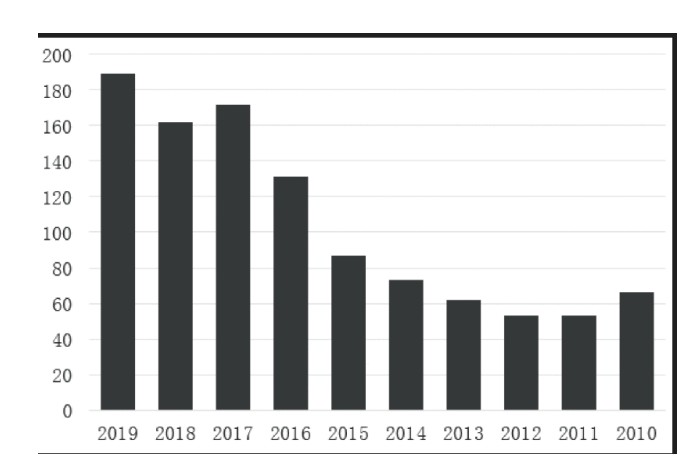
\includegraphics[width=.5\textwidth]{pic/picture_2.jpg}
		\caption{Papers in Web of Science and Google Scholar in the last ten year with key words “AI” and “Education”}
	\end{figure}
\end{frame}

\begin{frame}
\begin{itemize}
\item Diverse Roles of AI in Education:
This question investigates the multifaceted roles that AI assumes within education. It delves into how AI technologies are intricately linked with established educational and learning theories, while also examining the extent to which these technologies influence the processes of learning and instruction.
\item Addressing Research Questions:
In response to the research questions, the chosen articles are analyzed based on the educational and learning theories utilized to inform the design and implementation of AI technologies
  
   \end{itemize} 
\end{frame}

% Results --- --- --- --- --- --- --- --- --- --- --- 
\section{Results}
\begin{frame}
    \begin{itemize}
        \item AI helped personalize learning and gave students quick feedback
        \item Teachers saved time as AI handled tasks like grading and tracking progress
        \item Challenges like keeping student data safe and ensuring fair AI decisions were identified
        \item It was found that AI could help teachers but could not replace the human touch they provide
    \end{itemize}
\end{frame}
\section{Conclusion}
\begin{frame}{Conclusion}
    The primary aim of this study was to evaluate the influence of AI on
the field of education. Employing a qualitative research approach,
the study employed a literature review as its research design and
methodology. Through the analysis of journal articles, professional
publications, and conference reports, the study sought to achieve
its objective. The evolution of computers and related technologies
has paved the way for research and innovations that ultimately cul-
minated in the emergence of AI across various sectors. Particularly
noteworthy is the progression from personal computers to subse-
quent advancements that have elevated processing power, comput-
ing capabilities, and the integration of computer technologies into
diverse machines, equipment, and platforms. This trajectory has
driven the development and utilization of AI, which has demon-
strated a significant impact across the sectors it has touched.
\end{frame}

% --- Refference ---

\section{References}
% --- References Page 1 ---
\begin{frame}
\frametitle{References}
\begin{thebibliography}{10}
\bibitem{r1}
\alert{Chen, L., Chen, P., & Lin, Z. (2020)}
\newblock {Artificial intelligence in education: A review. Ieee Access, 8, 75264-75278.}

\bibitem{r2}
\alert{Harry, A. (2023)}
\newblock {Role of AI in Education. Interdisciplinary Journal and Humanity (INJURITY), 2(3), 260-268.}

\bibitem{r3}
\alert{Chan, C. K. Y., & Hu, W. (2023)}
\newblock {Students’ voices on generative AI: Perceptions, benefits, and challenges in higher education. International Journal of Educational Technology in Higher Education, 20(1), 43.}

\bibitem{r4}
\alert{Selwyn, N. (2022)}
\newblock {The future of AI and education: Some cautionary notes. European Journal of Education, 57(4), 620-631.}
\end{thebibliography}
\end{frame}

% --- References Page 2 ---
\begin{frame}
\frametitle{References}
\begin{thebibliography}{10}
\setcounter{enumiv}{4}
\bibitem{r5}
\alert{Chan, C. K. Y., & Tsi, L. H. (2023)}
\newblock {The AI revolution in education: Will AI replace or assist teachers in higher education?. arXiv preprint arXiv:2305.01185.}

\bibitem{r6}
\alert{Luckin, R., & Cukurova, M. (2019)}
\newblock {Designing educational technologies in the age of AI: A learning sciences‐driven approach. British Journal of Educational Technology, 50(6), 2824-2838.}

\bibitem{r7}
\alert{Conati, C., Porayska-Pomsta, K., & Mavrikis, M. (2018)}
\newblock {AI in Education needs interpretable machine learning: Lessons from Open Learner Modelling. arXiv preprint arXiv:1807.00154.}

\bibitem{r8}
\alert{Sok, S., & Heng, K. (2024)}
\newblock {Opportunities, challenges, and strategies for using ChatGPT in higher education: A literature review. Journal of Digital Educational Technology, 4(1), ep2401.}
\end{thebibliography}
\end{frame}

% --- References Page 3 ---
\begin{frame}
\frametitle{References}
\begin{thebibliography}{10}
\setcounter{enumiv}{8}
\bibitem{r9}
\alert{Qadir, J. (2023, May)}
\newblock {Engineering education in the era of ChatGPT: Promise and pitfalls of generative AI for education. In 2023 IEEE Global Engineering Education Conference (EDUCON) (pp. 1-9). IEEE.}

\bibitem{r10}
\alert{Marr, B. (2018)}
\newblock {How is AI used in education—Real world examples of today and a peek into the future. Forbes, Forbes Magazine, 25.}
\end{thebibliography}
\end{frame}


% --- Thank you slide ---
\begin{frame}
\begin{center}
{ Thank you for listening !}
\vspace{1cm}

Azizul Haque Tutul \\[1em]
(ID : 214052)
\end{center}
\end{frame}

\end{document}